\documentclass[xcolor=pdftex,dvipsnames]{beamer}

\usepackage{amsmath}
\usepackage{amssymb}

\usepackage{comment}
\usepackage{textcomp}

\title{Microeconomic Theory --- ECON 323 503 \\ Chapter 11: Monopoly
  and Monopsony}
\author{Vikram Manjunath}       %
\institute{Texas A\&M University}
\setbeamertemplate{navigation symbols}{}
\setbeamertemplate{footline}{}
\usefonttheme{serif}
\begin{document}

\maketitle

\begin{frame}
\frametitle{Outline}
\begin{enumerate}[<+->]
\item Monopoly profit maximization: still $MR=MC$. Just that $MR$ is
  different now.
\item Market power and welfare: Now, price will be higher than
  $MC$. So social welfare is diminished.
\item  Causes of monopolies: cost advantage of larger firms and
  government actions.
\item  Government actions that reduce market power: regulate the price
  or the help other firms enter the market.
\item Monopsony: single buyer rather than single seller.
\end{enumerate}
\end{frame}


\begin{frame}
  \frametitle{Monopoly profit maximization}
  Remember: at quantity $Q$,
  \[
  \pi(Q) = R(Q) - C(Q)
  \]

\uncover<2->{  First order condition:
\[
\frac{d\pi(Q)}{dQ} = \frac{dR(Q)}{dQ} - \frac{dC(Q)}{dQ} = 0
\]}
\uncover<3->{  In other words:
\[
MR(Q) = MC(Q)
\]}
\end{frame}

\begin{frame}
  \frametitle{Monopoly profit maximization}
Second order condition:
\[
\frac{d^2\pi(Q)}{dQ^2} = \frac{d^2R(Q)}{dQ^2} - \frac{d^2C(Q)}{dQ^2} < 0
\]
\uncover<2->{  $\frac{d^2R(Q)}{dQ^2} = \frac{dMR(Q)}{dQ}$ --- slope of MR curve}
\bigskip

\uncover<3->{  $\frac{d^2C(Q)}{dQ^2} = \frac{dMC(Q)}{dQ}$ --- slope of MC curve}

\uncover<4->{  So, second order condition says 
\[
\frac{dMR(Q)}{dQ} < \frac{dMC(Q)}{dQ}
\]}

\uncover<5->{In words: slope of  MR curve is less than slope of MC curve.}
\bigskip

\uncover<6->{  MC curve is either constant or upward sloping.}
\bigskip

\uncover<7->{  We'll see that MR is downward sloping.}
  
\end{frame}


\begin{frame}
  \frametitle{Marginal revenue and demand curves}
  Inverse demand: $p(Q)$ is the price that consumers pay when they buy
  $Q$ units.

\uncover<2->{\bigskip  So 
\[
R(Q) = p(Q)Q.
\]}

\uncover<3->{ Differentiating with respect to $Q$,
\[
MR(Q) = \frac{dR(Q)}{dQ} = 
p(Q) + \frac{dp(Q)}{dQ} Q
\]
}
\end{frame}


\begin{frame}
  \frametitle{Marginal revenue and demand curves}
\[ MR = p + \frac{dp}{dQ}Q\]
\uncover<2->{$p$ --- additional revenue from selling one more unit.}
\bigskip

\uncover<3->{$\frac{dp}{dQ}<0$ --- change (decrease) in price if you sell on more unit.}

\bigskip
\uncover<4->{$\frac{dp}{dQ}Q$ --- decrease in revenue due to price reduction.}

\bigskip
\uncover<5->{ The firm must consider the effect on the price of increased output.}


\bigskip
\uncover<6->{ Since $\frac{dp}{dQ}<0$, for every $Q$
\[
MR < p.
\]}
\uncover<7->{ So $MR$ curve is \emph{below} the demand curve.}

\end{frame}

\begin{frame}
  \frametitle{Comparison with competitive firm}
  Remember that competitive firms face perfectly elastic demand.
\bigskip

\uncover<2->{ So for a competitive firm $p(Q)$ is constant.}
\bigskip

\uncover<3->{ This means $\frac{dp}{dQ} = 0$ so $MR = p$.}
\bigskip

\uncover<4->{ So for a competitive firm $MR$ curve coincides with the demand curve.}
\end{frame}


\begin{frame}
  \frametitle{Graphical illustration}
  \begin{center}
    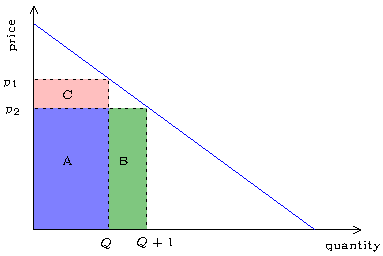
\includegraphics{pics/MR}
  \end{center}

\uncover<2->{$C$ --- lost revenue on the first $Q$ units. }
\smallskip 

\uncover<3->{$B$ --- revenue gained by selling the last unit.}
\[\uncover<4->{MR = (A+B) - (A+C) }\uncover<5->{= B - C} \uncover<6->{= p_2 - C}\uncover<7->{ = p_2  - \frac{dp}{dQ}Q}\]
\end{frame}




\begin{frame}
  \frametitle{Marginal revenue and the elasticity of demand}
  The slope of demand ($\frac{dp}{dQ}$) is important in determining $MR$.
\bigskip

\uncover<2->{This is closely related to the elasticity of demand.}

\[
\begin{array}{rcl}
\uncover<3->{MR &=& p + \frac{dp}{dQ}Q\\\\}
\uncover<4->{  &=& p\left(1 + \frac{dp}{dQ}\frac{Q}{p} \right)\\\\}
\uncover<5->{  &=&  p\left(1 + \dfrac{1}{\frac{dQ}{dp}\frac{p}{Q}}\right)\\\\}
\uncover<6->{  &=&  p\left(1+\frac{1}{\varepsilon}\right)}
\end{array}
\]
\uncover<7->{Again, as $\varepsilon\to -\infty$ (competitive firm), $MR\to p$.}

\end{frame}
\begin{frame}
  \frametitle{An example}
  \[
  p(Q) = 24 - Q
  \]
\uncover<2->{  \[
\frac{dp}{dQ} = -1
\]}
\[
\begin{array}{rcl}
\uncover<3->{  MR(Q) &=& p(Q) + \frac{dp}{dQ}Q}\\\\\uncover<4->{ &=&
  (24-Q) + (-1)Q}\\\\\uncover<5->{ &=& 24 -2Q   }
\end{array}
\]
\uncover<6->{Notice that except when $Q>0$, $MR(Q) < P(Q)$.}
\end{frame}

\begin{frame}
  \frametitle{An example}
  \begin{center}
    \includegraphics{pics/MRExample1}
  \end{center}
When $Q=0$,  $\varepsilon = -\infty$ so $MR(Q) = p(Q) = 24$.
\end{frame}
\begin{frame}
  \frametitle{An example}
  \begin{center}
    \includegraphics{pics/MRExample2}
  \end{center}
When $Q=12$,   $\varepsilon = -1$ so $MR(Q) = 0$!
\end{frame}

\begin{frame}
  \frametitle{Implication of elastic demand}
From the picture: For $Q$ where demand is inelastic, MR is
\emph{negative}.
\bigskip

\uncover<2->{ So the firm's revenue decreases with every additional unit that it
produces.}

\bigskip

\uncover<3->{ Mathematically, we saw that
\[
MR = p\left(1+\frac{1}{\varepsilon}\right).
\]}
\uncover<4->{ If $\varepsilon > -1$, MR is negative.}

\bigskip
\uncover<5->{ Implication: A monopolist \emph{never} produces a quantity where
demand is inelastic!}
\end{frame}


\begin{frame}
  \frametitle{Monopoly profit maximization}
  Recall that the firm picks $Q^*$ so that 
\[
MR(Q^*) = MC(Q*).
\]
\uncover<2->{ For competitive firms, $MR(Q^*) = p$ so the MC curve \emph{is} the
supply curve.}

\bigskip
\uncover<3->{ What about for a monopolist?}

\bigskip
\uncover<4->{ Still set $MR = MC$.}

\bigskip
\uncover<5->{ Example: $C(Q) = Q^2 + 12$. Then
\[MC(Q) = \frac{dC}{dQ} = 2Q.\]}

\uncover<6->{ Firm looks for  $Q^*$ such that
\[
MR(Q^*) = 24-2Q^* = 2Q^* = MC(Q^*).
\]}
\uncover<7->{ Solving this, 
\[
Q^* = 6.
\]}
\end{frame}

\begin{frame}
  \frametitle{Graphical illustration}
  \begin{center}
    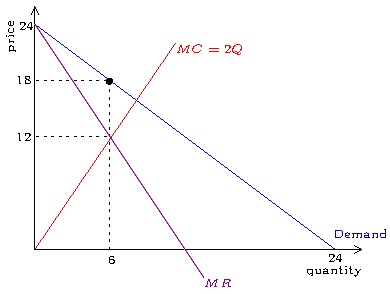
\includegraphics{pics/MonopProf1}
  \end{center}
Demand not perfectly elastic so MR curve is not horizontal.\\
\uncover<2->{ Determine $Q$ by equating $MR$ and $MC$. \\}
\uncover<3->{ Demand curve gives us the price.}
\end{frame}
\begin{frame}
  \frametitle{Graphical illustration}
  \begin{center}
    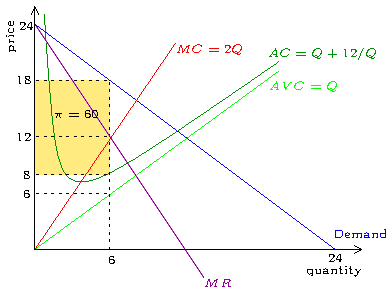
\includegraphics{pics/MonopProf2}
  \end{center}
$AC(Q) = \frac{C(Q)}{Q} = Q+\frac{12}{Q}$.\\
\uncover<2->{$AVC(Q) = \frac{VC(Q)}{Q} = Q$.}
\uncover<3->{ Since $AC(Q^*) = 8< 18 = p^* $, firm makes a positive profit.}

\end{frame}


\begin{frame}
  \frametitle{Shut down decision}
  The shutdown decision for the monopolist is just like that of a
  competitive firm.
\bigskip

\uncover<2->{ Short run: shut down if monopoly price  less than AVC.}
\bigskip

\uncover<3->{ Long run: shut down if monopoly price less than AC.}
\end{frame}

\begin{frame}
  \frametitle{Price or quantity?}
  Does the firm get to decide price or quantity?
\bigskip

\uncover<2->{ It doesn't matter. }
\bigskip

\uncover<3->{ If the firm picks a price $p$, then it's effectively picking the
quantity $Q(p)$.}
\bigskip

\uncover<4->{ If the firm picks a quantity $Q$, then it's effectively picking the
price $p(Q)$.}

\bigskip

\uncover<5->{ Remember that we can derive the function $p()$ from the function $Q()$
and vice versa.}
\end{frame}




\begin{frame}
  \frametitle{What happens if demand shifts?}
  \begin{center}
    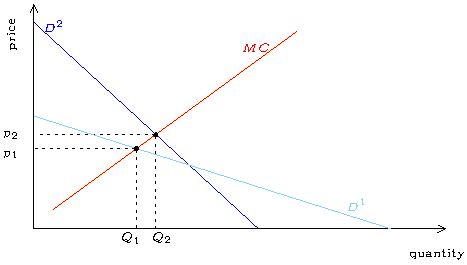
\includegraphics{pics/ShiftComp}
  \end{center}
  Competitive firms: MC curve is the supply curve.\\
  So there's a one-to-one relationship between equilibrium prices and quantities.
\end{frame}

\begin{frame}
  \frametitle{What happens if demand shifts?}
  \begin{center}
    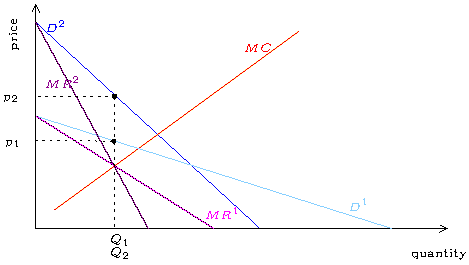
\includegraphics{pics/ShiftMon} 
  \end{center}
  Monopolist: No well-defined supply curve.
  When demand shifts, quantity remains the same, but price
  increases. No one-to-one relationship between price and quantity.
\end{frame}


\begin{frame}
  \frametitle{Market power and welfare}
  Monopolists are \emph{not} price-takers. They\emph{can} affect the
  price to earn a \emph{positive} profit.
\bigskip

\uncover<2->{They \emph{don't} set the price at MC.}
\bigskip

\uncover<3->{  This is called \emph{market power}.}
\bigskip

\uncover<4->{\[
MR = p\left(1+\frac{1}{\varepsilon}\right) = MC
\]}
\uncover<5->{ Rearranging,
\[
\frac{p}{MC} = \dfrac{1}{1+\frac{1}{\varepsilon}}.
\]}
\uncover<6->{ This the ratio of the price to marginal cost.}
\bigskip

\uncover<7->{ For competitive firms, $\frac{p}{MC} = 1$.}
\bigskip

\uncover<8->{ The higher this ratio, the more the firm is paid above its marginal cost.}
\end{frame}

\begin{frame}
  \frametitle{The Lerner Index}
  The Lerner index is the markup in the price of a good: the
  proportion of the price that goes towards profits of the firm as
  opposed to costs: $\frac{p-MC}{p}$.


\uncover<2->{ Since $\frac{p}{MC} = \dfrac{1}{1+\frac{1}{\varepsilon}}$, 
\[
\frac{MC}{p}= 1+ \frac{1}{\varepsilon}.
\]}

\uncover<3->{ So 
\[
\frac{p-MC}{p} = 1-\frac{MC}{p} = -\frac{1}{\varepsilon}.
\]}

\end{frame}


\begin{frame}
  \frametitle{Sources of market power}
  The more \emph{inelastic} demand is, the greater the market power.

\uncover<2->{  Demand is less elastic (more inelastic) when }
  \begin{enumerate}
  \item<3-> There are fewer substitutes.
  \item<4-> There are fewer firms selling the same product.
  \end{enumerate}

\end{frame}

\begin{frame}
  \frametitle{Effect of market power on welfare}
  What happens to $W=CS+PS$ when a firm has market power?
\bigskip

\uncover<2->{ There's deadweight loss.}

\bigskip

\uncover<3->{ The monopolist produces too little of the good.}
\end{frame}

\begin{frame}
  \frametitle{Deadweight loss from monopoly}
  \begin{center}
    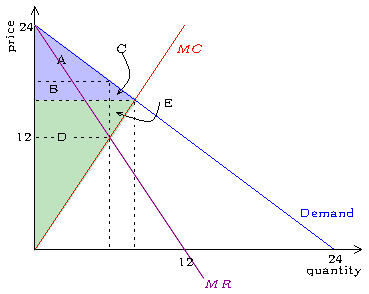
\includegraphics{pics/DWLc}

  {\scriptsize
    \begin{tabular}{lccc}
\hline      & Competition & Monopoly & Change\\
\hline      CS & A+B+C &{\color{white} A }&{\color{white} -B-C}\\
\hline      PS & D + E &{\color{white}  D+ B} & {\color{white}  B-E} \\
\hline      W & A+B+C+D+E & {\color{white} A+B+D} & {\color{white} -C-E = DWL}\\\hline
    \end{tabular}
  }
  \end{center}\end{frame}
\begin{frame}
  \frametitle{Deadweight loss from monopoly}
  \begin{center}
    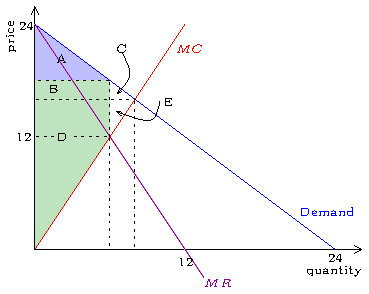
\includegraphics{pics/DWLm}

  {\scriptsize
    \begin{tabular}{lccc}
\hline      & Competition & Monopoly & Change\\
\hline      CS & A+B+C &A &{\color{white} -B-C}\\
\hline      PS & D + E & D+ B & {\color{white}  B-E} \\
\hline      W & A+B+C+D+E &  A+B+D & {\color{white} -C-E = DWL}\\\hline
    \end{tabular}
  }
  \end{center}\end{frame}

\begin{frame}
  \frametitle{Deadweight loss from monopoly}
  \begin{center}
    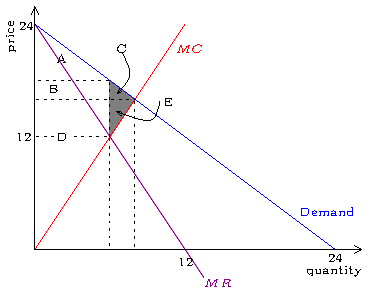
\includegraphics{pics/DWL}

  {\scriptsize
    \begin{tabular}{lccc}
\hline      & Competition & Monopoly & Change\\
\hline      CS & A+B+C &A &{-B-C}\\
\hline      PS & D + E & D+ B &  B-E \\
\hline      W & A+B+C+D+E &  A+B+D &  -C-E = DWL\\\hline
    \end{tabular}
  }
  \end{center}\end{frame}



\begin{frame}
  \frametitle{Causes of monopolies}
  \begin{enumerate}
  \item A firm might own a scarse resource (an \emph{essential facility}).

  \item<2-> It may just have better technology so that it can produce
    at a lower cost than any potential rival.
\item <3-> Licenses/patents  and other barriers to entry.
  \item<4-> It's a ``natural monopoly.''
  \end{enumerate}
\end{frame}

\begin{frame}
  \frametitle{Natural monopolies}
  Let 
\[
Q = q_1 + q_2 + \dots q_n
\]
\uncover<2->{
If $n$ different firms produces these different amounts, total cost: 
\[
c(q_1)   + c(q_2) + \dots + c(q_n)
\]
}
\uncover<3->{
If one firm produces all of it, total cost is $c(Q)$.}

\bigskip
\uncover<4->{\emph{Natural monopoly:}
\[
c(q_1)   + c(q_2) + \dots + c(q_n) > c(Q)
\]}
\uncover<5->{It's cheaper for one firm to produce all of it than for several firms
to produce parts of it.}

\end{frame}


\begin{frame}
  \frametitle{Utilities}
  Common example of natural monopoly: utilities.

\bigskip

\uncover<2->{$F$ --- cost of building supply infrastructure}
\bigskip

\uncover<3->{$m$ --- cost of connecting supplying to a home}
\bigskip

\uncover<4->{$m$ is the constant marginal cost. }
\bigskip

\uncover<5->{\[AC = m+\frac{F}{Q}\]}

\uncover<6->{$AC$ is diminishing in $Q$}

\end{frame}



\begin{frame}
  \frametitle{Utilities}
  
  \begin{center}
    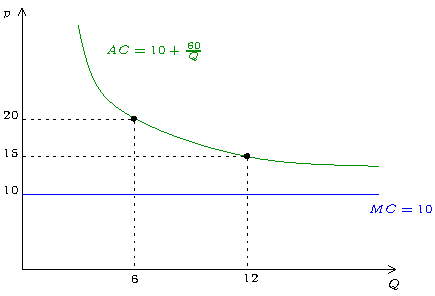
\includegraphics{pics/NatMon}
  \end{center}
MC is the same no matter how many firms. So the most efficient way to
produce is to have only one firm. 
\end{frame}

\begin{frame}
  \frametitle{Utilities}
  
  \begin{center}
    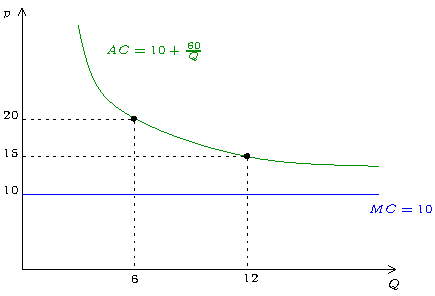
\includegraphics{pics/NatMon}
  \end{center}
AC for one firm producing 12 units is 15.\\
AC for two firms each producing 6 units is 20.
\end{frame}

\begin{frame}
  \frametitle{Utilities}
  
  \begin{center}
    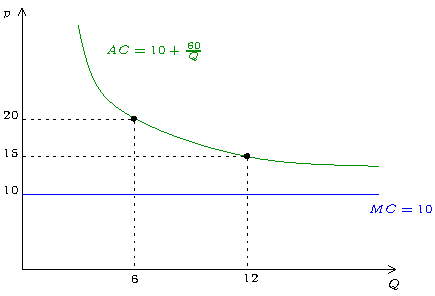
\includegraphics{pics/NatMon}
  \end{center}
If the firm sets its price at MC, it can't stay in business in the
long run.
\end{frame}





\begin{frame}
  \frametitle{Government actions to redue market power}
\emph{  Optimal price regulation:} \uncover<2->{Remember price ceilings?}

\uncover<3->{\bigskip
They cause welfare losses when used improperly (in competitive
markets).}

\bigskip
\uncover<4->{ But they can save the day with monopolies.}

\bigskip
\uncover<5->{ Just set the price ceiling at the equilibrium price if there market
\emph{had been} competitive: where $D = MC$.}

\end{frame}


\begin{frame}
  \frametitle{Optimal price regulation}
  \begin{center}
    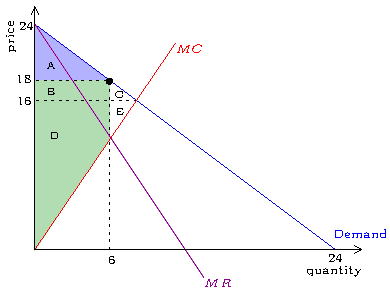
\includegraphics{pics/OptReg1}

  {\scriptsize
    \begin{tabular}{lccc}
\hline      & No Regulation & Regulation & Change\\
\hline      CS & A&{\color{white}A+B+C} &{\color{white}{B+C}}\\
\hline      PS & B+D  & {\color{white}D+ E} &  {\color{white}E-B} \\
\hline      W & A+B+D &  {\color{white}A+B+C+D+E} &  {\color{white}C+E = $\Delta$DWL}\\\hline
    \end{tabular}
  }
  \end{center}
\end{frame}




\begin{frame}
  \frametitle{Optimal price regulation}
  \begin{center}
    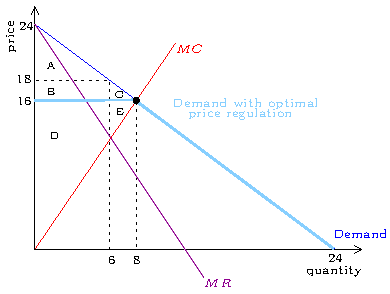
\includegraphics{pics/OptReg2}

  {\scriptsize
    \begin{tabular}{lccc}
\hline      & No Regulation & Regulation & Change\\
\hline      CS & A&{\color{white}A+B+C} &{\color{white}{B+C}}\\
\hline      PS & B+D  & {\color{white}D+ E} &  {\color{white}E-B} \\
\hline      W & A+B+D &  {\color{white}A+B+C+D+E} &  {\color{white}C+E = $\Delta$DWL}\\\hline
    \end{tabular}
  }
  \end{center}
\end{frame}


\begin{frame}
  \frametitle{Optimal price regulation}
  \begin{center}
    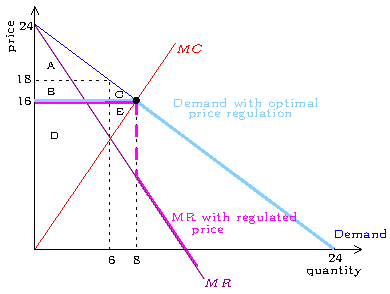
\includegraphics{pics/OptReg3}

  {\scriptsize
    \begin{tabular}{lccc}
\hline      & No Regulation & Regulation & Change\\
\hline      CS & A&{\color{white}A+B+C} &{\color{white}{B+C}}\\
\hline      PS & B+D  & {\color{white}D+ E} &  {\color{white}E-B} \\
\hline      W & A+B+D &  {\color{white}A+B+C+D+E} &  {\color{white}C+E = $\Delta$DWL}\\\hline
    \end{tabular}
  }
  \end{center}
\end{frame}







\begin{frame}
  \frametitle{Optimal price regulation}
  \begin{center}
    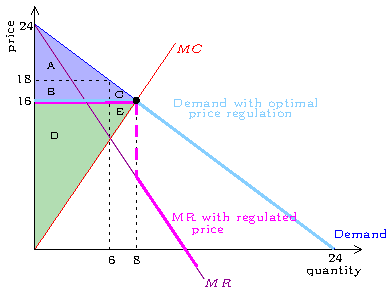
\includegraphics{pics/OptReg4}

  {\scriptsize
    \begin{tabular}{lccc}
\hline      & No Regulation & Regulation & Change\\
\hline      CS & A&{A+B+C} &{\color{white}{B+C}}\\
\hline      PS & B+D  & {D+ E} &  {\color{white}E-B} \\
\hline      W & A+B+D &  {A+B+C+D+E} &  {\color{white}C+E = $\Delta$DWL}\\\hline
    \end{tabular}
  }
  \end{center}
\end{frame}

\begin{frame}
  \frametitle{Optimal price regulation}
  \begin{center}
    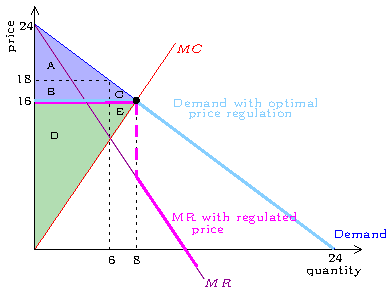
\includegraphics{pics/OptReg4}

  {\scriptsize
    \begin{tabular}{lccc}
\hline      & No Regulation & Regulation & Change\\
\hline      CS & A&{A+B+C} &{{B+C}}\\
\hline      PS & B+D  & {D+ E} &  {E-B} \\
\hline      W & A+B+D &  {A+B+C+D+E} &  {C+E = $\Delta$DWL}\\\hline
    \end{tabular}
  }
  \end{center}
\end{frame}


\begin{frame}
  \frametitle{What if the regulation isn't optimal?}
  \begin{itemize}
  \item If the regulated price is too high: still have a deadweight
    loss from monopoly's market power.
  \item<2-> If the regulated price is a little too low: deadweight loss from
    ``over consumption'' of the good.
  \item<3-> If the regulated price is really low (below the firm's
    minimum AC), the firm goes out of business causing a high
    deadweight loss.
  \end{itemize}
\end{frame}

\begin{frame}
  \frametitle{Difficulties in regulating}
  \begin{enumerate}
  \item Hard to know exactly what the demand and marginal cost curves are.

  \item<2-> Regulator's are often \emph{captured.} Unfortunately the
    industry being regulated is often able to influence regulators.
  \item<3-> If the monopoly can't be subsidized, setting the price
    equal at MC can cause firms to go out of business or not enter.
  \end{enumerate}
\end{frame}


\begin{frame}
  \frametitle{Monopsony}
  The scenario is flipped: only one buyer and many sellers.

  \bigskip
\uncover<2->{  Examples: Professional sports leagues are the only ``consumers'' of
  the labor provided by athletes. }

\uncover<3->{  \bigskip
  Monopoly $\to$ price too high.
  \bigskip}
  
\uncover<4->{  Monopsony $\to$ price too low.}

  \bigskip
\uncover<5->{  Either way, quantity too low so deadweight loss.}
\end{frame}


\begin{frame}
  \frametitle{Monopsony and profit maximization}
  Think of a town with only one big employer.
  
  \bigskip
\uncover<2->{  It's a monopsony in the labor market.}
  \bigskip

\uncover<3->{   Inverse supply function: $w(L)$ is the price at which $L$ units of labor
  are supplied.}\uncover<4->{  Assume that this is upward sloping.}

  \bigskip
\uncover<5->{   What happens to its expenditure ($Lw$) if the monopsony hires one more unit
  of labor?}

\uncover<6->{   \[
  ME = \underset{\text{price of extra unit}}{w(L)} +
  \underset{\text{increased wages paid for existing units}}{\frac{dw}{dL}L}.
  \]}

\end{frame}

\begin{frame}
  \frametitle{Comparison with competitive market}
  If the labor market were competitive, there would be many other employers.

  \bigskip
\uncover<2->{  Then $\frac{dw}{dL}$ would be 0, so $ME$ would be $p$.}

  \bigskip
\uncover<3->{  (Just like monopoly.)}
\end{frame}

\begin{frame}
  \frametitle{Monopsony and profit maximization}
  How much labor should the employer hire?

  \bigskip
\uncover<2->{  Remember  $D(L)$ tells us how much the $L^{\text{th}}$ unit of labor
  is worth to the employer.}


  \bigskip
\uncover<3->{  Whether competitive of monopsony, pick $L$ such that:
  \[
  ME(L)  = D(L).
  \]}
\uncover<4->{ Why?}
\end{frame}


\begin{frame}
  \frametitle{Monopsony power}
  Can write down the Lerner index just as before:
  \[
  \frac{ME-w}{w} = \frac{1}{\eta}
\]

\uncover<2->{ Monopsony power has deadweight loss too. }
\bigskip

\uncover<3->{ The higher the monopsony power, the higher the deadweight loss.}

\bigskip
\uncover<4->{ So, the less elastic supply is, the more the deadweight loss because
of a monopsony.}

\end{frame}






\end{document}








